% $Header: /home/vedranm/bitbucket/beamer/solutions/generic-talks/generic-ornate-15min-45min.en.tex,v 90e850259b8b 2007/01/28 20:48:30 tantau $
\documentclass{beamer}
%\documentclass[handout]{beamer}
\usefonttheme[onlymath]{serif}
% This file is a solution template for:
\usepackage{algorithm}
\usepackage{algpseudocode}
\usepackage{multicol}
% - Giving a talk on some subject.
% - The talk is between 15min and 45min long.
% - Style is ornate.



% Copyright 2004 by Till Tantau <tantau@users.sourceforge.net>.
%
% In principle, this file can be redistributed and/or modified under
% the terms of the GNU Public License, version 2.
%
% However, this file is supposed to be a template to be modified
% for your own needs. For this reason, if you use this file as a
% template and not specifically distribute it as part of a another
% package/program, I grant the extra permission to freely copy and
% modify this file as you see fit and even to delete this copyright
% notice. 

\mode<presentation>
{
  \usetheme{Warsaw}
  % or ...

  \setbeamercovered{transparent}
  % or whatever (possibly just delete it)
}
\setbeamertemplate{navigation symbols}{} 

\usepackage[english]{babel}
% or whatever

\usepackage[latin1]{inputenc}
% or whatever
\useoutertheme{default}

\usepackage{times}
\usepackage[T1]{fontenc}
% Or whatever. Note that the encoding and the font should match. If T1
% does not look nice, try deleting the line with the fontenc.
\newcommand{\beforeverb}{\footnotesize}
\newcommand{\afterverb}{\normalsize}

\title[Iterative Methods For Linear Algebra ] % (optional, use only with long paper titles)
{Lecture 9}

\subtitle
{Iterative Methods For Linear Algebra } % (optional)

\author[Ying-Jer Kao] % (optional, use only with lots of authors)
{Ying-Jer Kao}
% - Use the \inst{?} command only if the authors have different
%   affiliation.

\institute[National Taiwan University] % (optional, but mostly needed)
{
  Department of Physics\\
 National Taiwan University
  }
% - Use the \inst command only if there are several affiliations.
% - Keep it simple, no one is interested in your street address.

\date[Numerical Analysis and Programming] % (optional)
{\today}

\subject{Talks}
% This is only inserted into the PDF information catalog. Can be left
% out. 



% If you have a file called "university-logo-filename.xxx", where xxx
% is a graphic format that can be processed by latex or pdflatex,
% resp., then you can add a logo as follows:

% \pgfdeclareimage[height=0.5cm]{university-logo}{university-logo-filename}
% \logo{\pgfuseimage{university-logo}}



% Delete this, if you do not want the table of contents to pop up at
% the beginning of each subsection:
%\AtBeginSubsection[]
%{
%  \begin{frame}<beamer>{Outline}
%    \tableofcontents[currentsection,currentsubsection]
%  \end{frame}
%}


% If you wish to uncover everything in a step-wise fashion, uncomment
% the following command: 

%\beamerdefaultoverlayspecification{<+->}


\begin{document}

\begin{frame}
  \titlepage
\end{frame}

\begin{frame}{Outline}
  \tableofcontents
  % You might wish to add the option [pausesections]
\end{frame}


% Since this a solution template for a generic talk, very little can
% be said about how it should be structured. However, the talk length
% of between 15min and 45min and the theme suggest that you stick to
% the following rules:  

% - Exactly two or three sections (other than the summary).
% - At *most* three subsections per section.
% - Talk about 30s to 2min per frame. So there should be between about
%   15 and 30 frames, all told.
\section[Introduction]{Introduction}
\subsection{Sparse Matrices}
\begin{frame}{Sparse Matrices}
    \begin{itemize}
        \item In many applications, the matrices are sparse, i.e., most of the elements are zero.
        \item For example, the adjacency matrix of a graph is sparse.
        \item The storage and computation of sparse matrices can be done efficiently using sparse matrix formats.
        \item The most common sparse matrix formats are the Compressed Sparse Row (CSR)
         and Compressed Sparse Column (CSC) formats.
    \end{itemize}
\end{frame}
\begin{frame}{Sparse Matrices}
    \begin{itemize}
        \item A \textbf{sparse matrix} is a matrix with a large proportion of zero elements.
        \item Need for Sparse Storage:
        \begin{itemize}
        \item Reduces memory usage
        \item Improves computational efficiency
        \end{itemize}
        \item Applications: Machine learning, scientific computing, graph algorithms
    \end{itemize}
\end{frame}
\begin{frame}{Example: Adjacency matrix}
\centerline{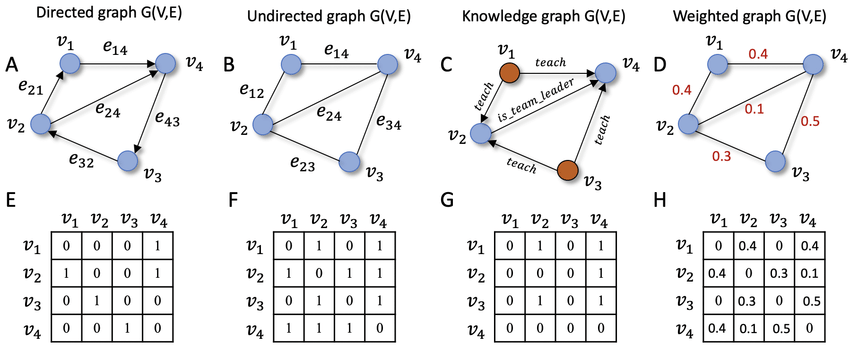
\includegraphics[width=\textwidth]{Different-types-of-graphs-and-their-corresponding-adjacency-matrix-representations-The.ppm.png}}
\end{frame}
\begin{frame}{Example: Tight-Binding Hamiltonian}
    \begin{itemize}
        \item The tight-binding Hamiltonian for a 1D chain of $N$ atoms 
        \[
        \mathbf{H}=-t \sum_{i=1}^{N-1} \left({c}_i^{\dagger} {c}_{i+1}+{c}_{i+1}^{\dagger} {c}_i\right)+
        \epsilon \sum_{i=1}^N {c}_i^{\dagger} {c}_i
        \]
        \item In the atomic basis, the Hamiltonian is represented by a matrix
        \[  
        H=\left[\begin{array}{llllllll}
        \epsilon & -t & 0 & 0 & \cdots & \cdots & \cdots & 0 \\
        -t & \epsilon & -t & 0 & \cdots & \cdots & \cdots & 0\\
        0 & -t & \epsilon & -t & \cdots & \cdots & \cdots & 0  \\
        \vdots & \cdots & \ddots & \ddots & \ddots & \cdots & \cdots &  0 \\
        \vdots & \cdots &  \cdots & \cdots & 0 & -t & \epsilon & -t \\
        0 & \cdots& \cdots & \cdots & \cdots &  0 & -t & \epsilon   
        \end{array}\right],
        \]
        which is a tridiagonal matrix.
    \end{itemize}
\end{frame}
\begin{frame}{Sparse Matrices}
    \begin{itemize}
    \item A sparse matrix 
        
    \[\left[\begin{array}{llllllllll}
       1 & 0 & 3 & 0 & 9 & 0 & 3 & 0 & 0 & 0 \\
       11 & 0 & 4 & 0 & 0 & 0 & 0 & 0 & 2 & 1 \\
       0 & 0 & 1 & 0 & 0 & 0 & 4 & 0 & 1 & 0 \\
       8 & 0 & 0 & 0 & 3 & 1 & 0 & 0 & 0 & 0 \\
       0 & 0 & 0 & 9 & 0 & 0 & 1 & 0 & 17 & 0 \\
       13 & 21 & 0 & 9 & 2 & 47 & 1 & 81 & 21 & 9 \\
       0 & 0 & 0 & 0 & 0 & 0 & 0 & 0 & 0 & 0 \\
       0 & 0 & 0 & 0 & 19 & 8 & 16 & 0 & 0 & 55 \\
       54 & 4 & 0 & 0 & 0 & 11 & 0 & 0 & 0 & 0 \\
       0 & 0 & 2 & 0 & 0 & 0 & 0 & 22 & 0 & 21 
        \end{array}\right]
    \] contains mostly zeros.
    \item We do not want to save zeros.
\end{itemize}
\end{frame}
\begin{frame}{Storing Sparse Matrices}
    \begin{itemize}
        \item A sparse matrix can be stored in a more efficient way.
        \item The most common sparse matrix formats are the Compressed Sparse Row (CSR) and Compressed Sparse Column (CSC) formats.
        \item The CSR format stores the matrix as three arrays: \texttt{values}, \texttt{columns}, and \texttt{row\_ptr}.
        \item The CSC format stores the matrix as three arrays: \texttt{values}, \texttt{rows}, and \texttt{col\_ptr}.
    \end{itemize}
\end{frame}
\begin{frame}{Coordinate (COO) Format}
    \begin{itemize}
        \item In the COO format, the matrix is stored as three arrays: \texttt{values}, \texttt{rows}, and \texttt{columns}.
    \end{itemize}
    \centerline{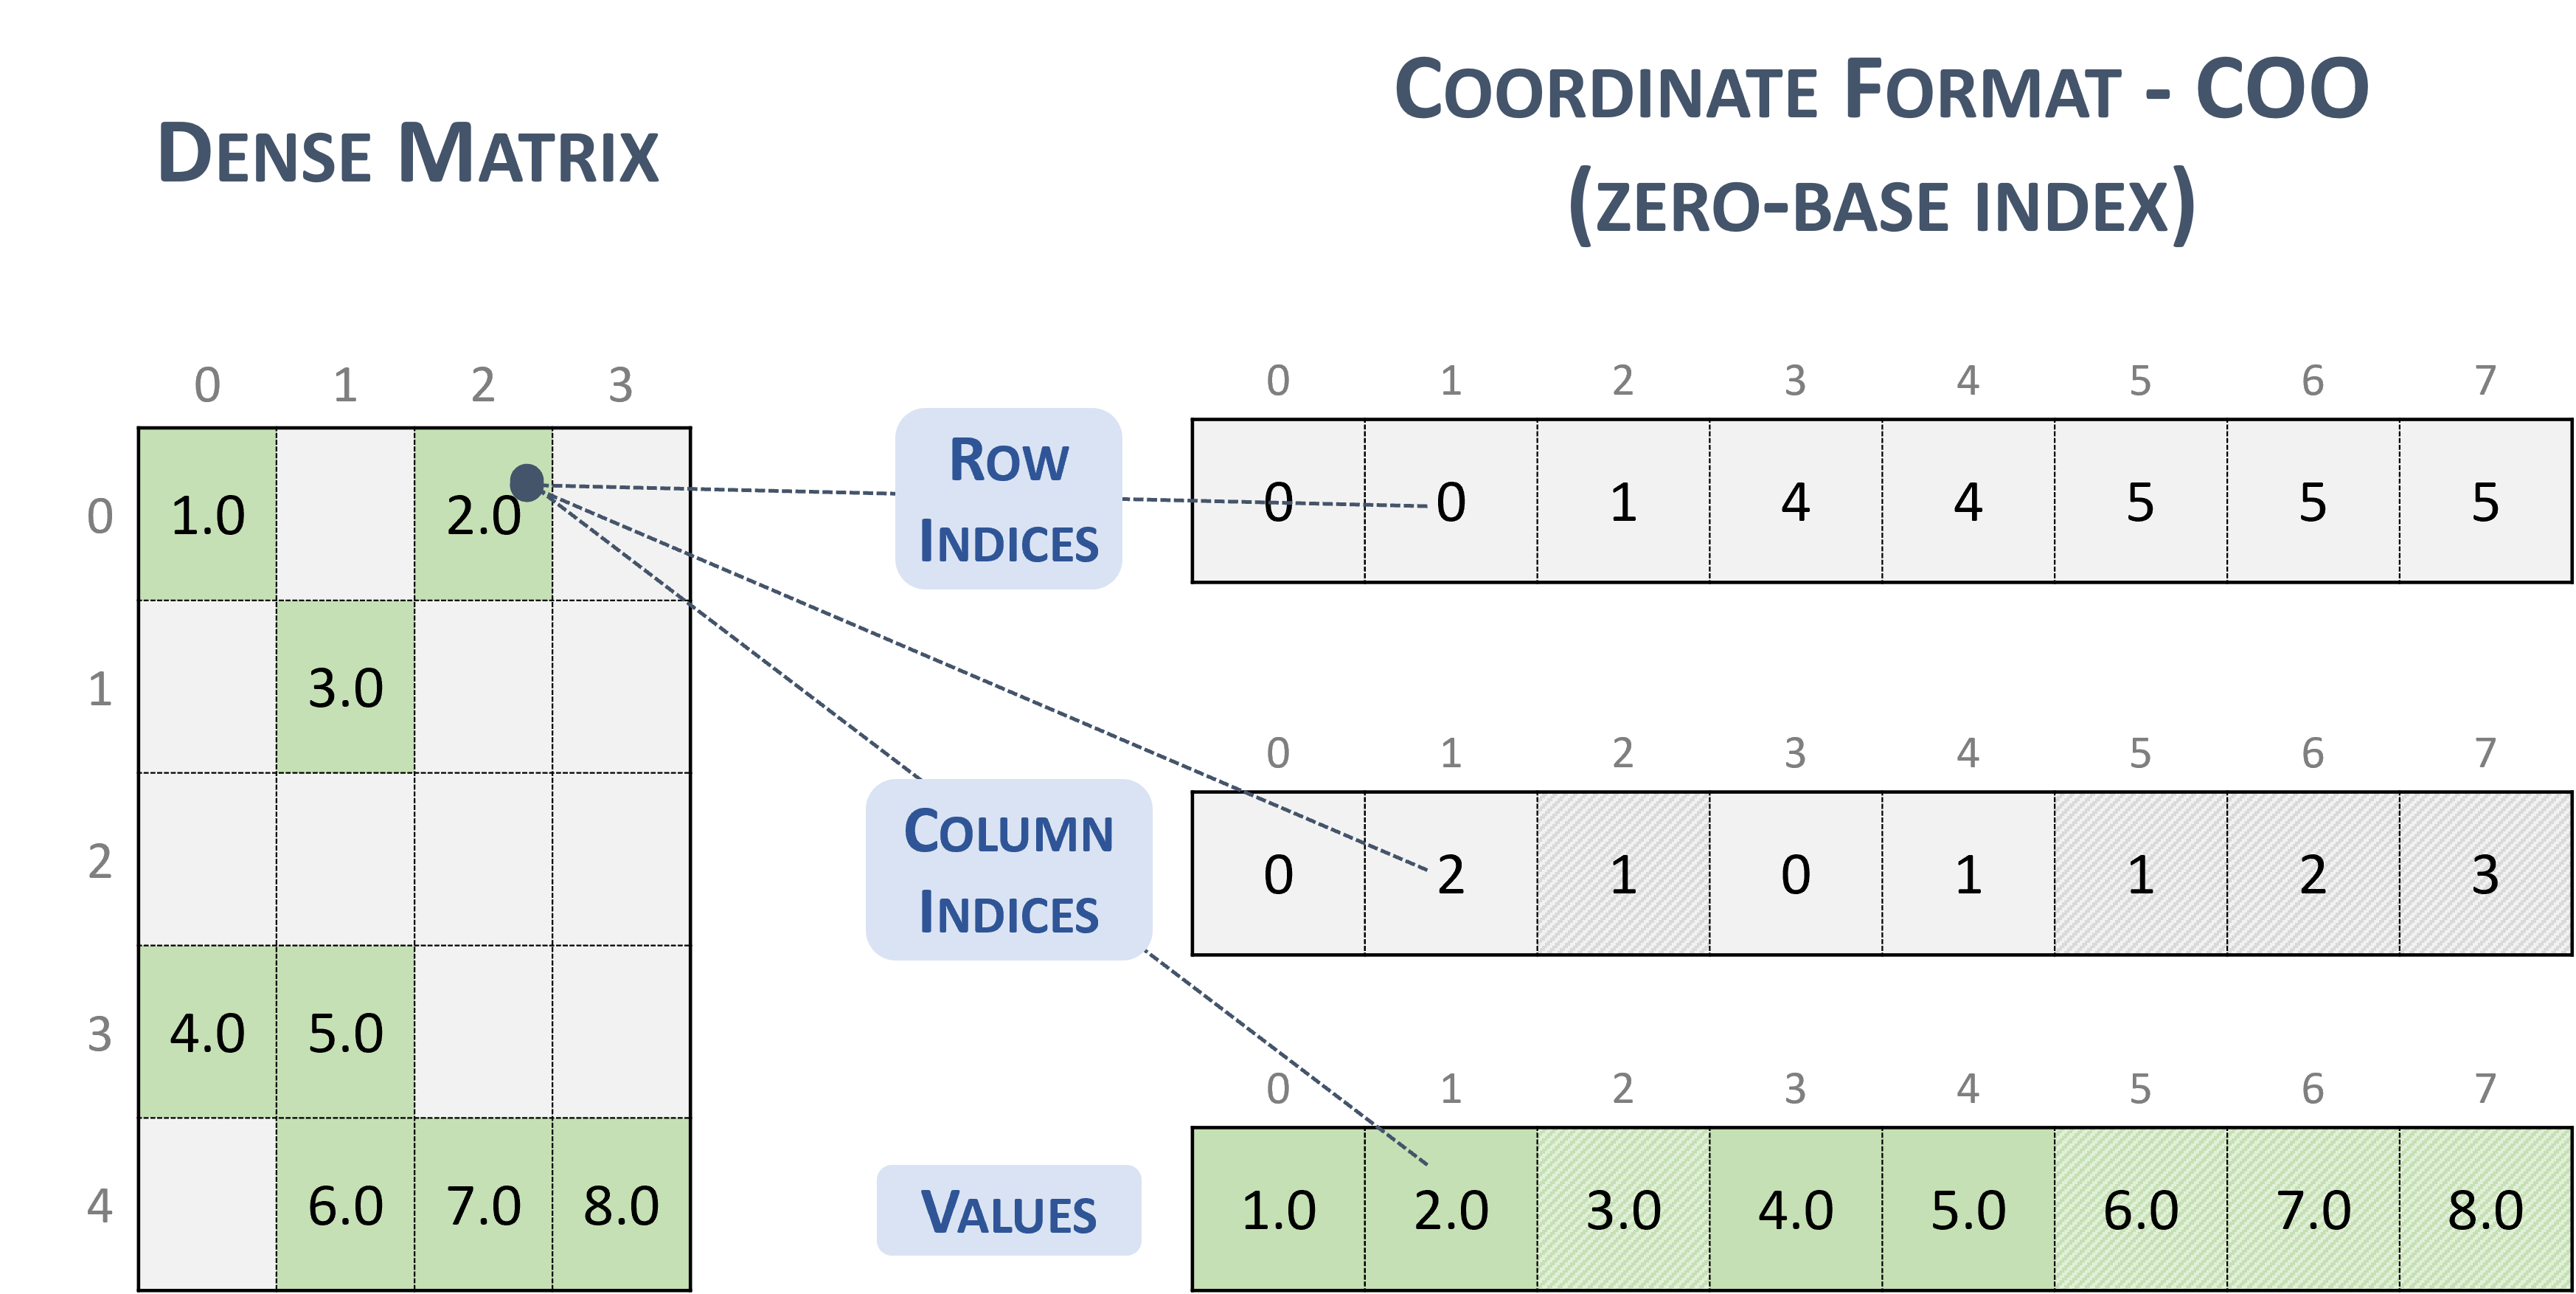
\includegraphics[width=\textwidth]{coo.png}}

\end{frame}
\begin{frame}{Compressed Sparse Row (CSR) Format}
    \begin{itemize}
        \item In the CSR format, the matrix is stored as three arrays: \texttt{values}, \texttt{columns}, and \texttt{row\_ptr}.
     
    \end{itemize}
    \centerline{ 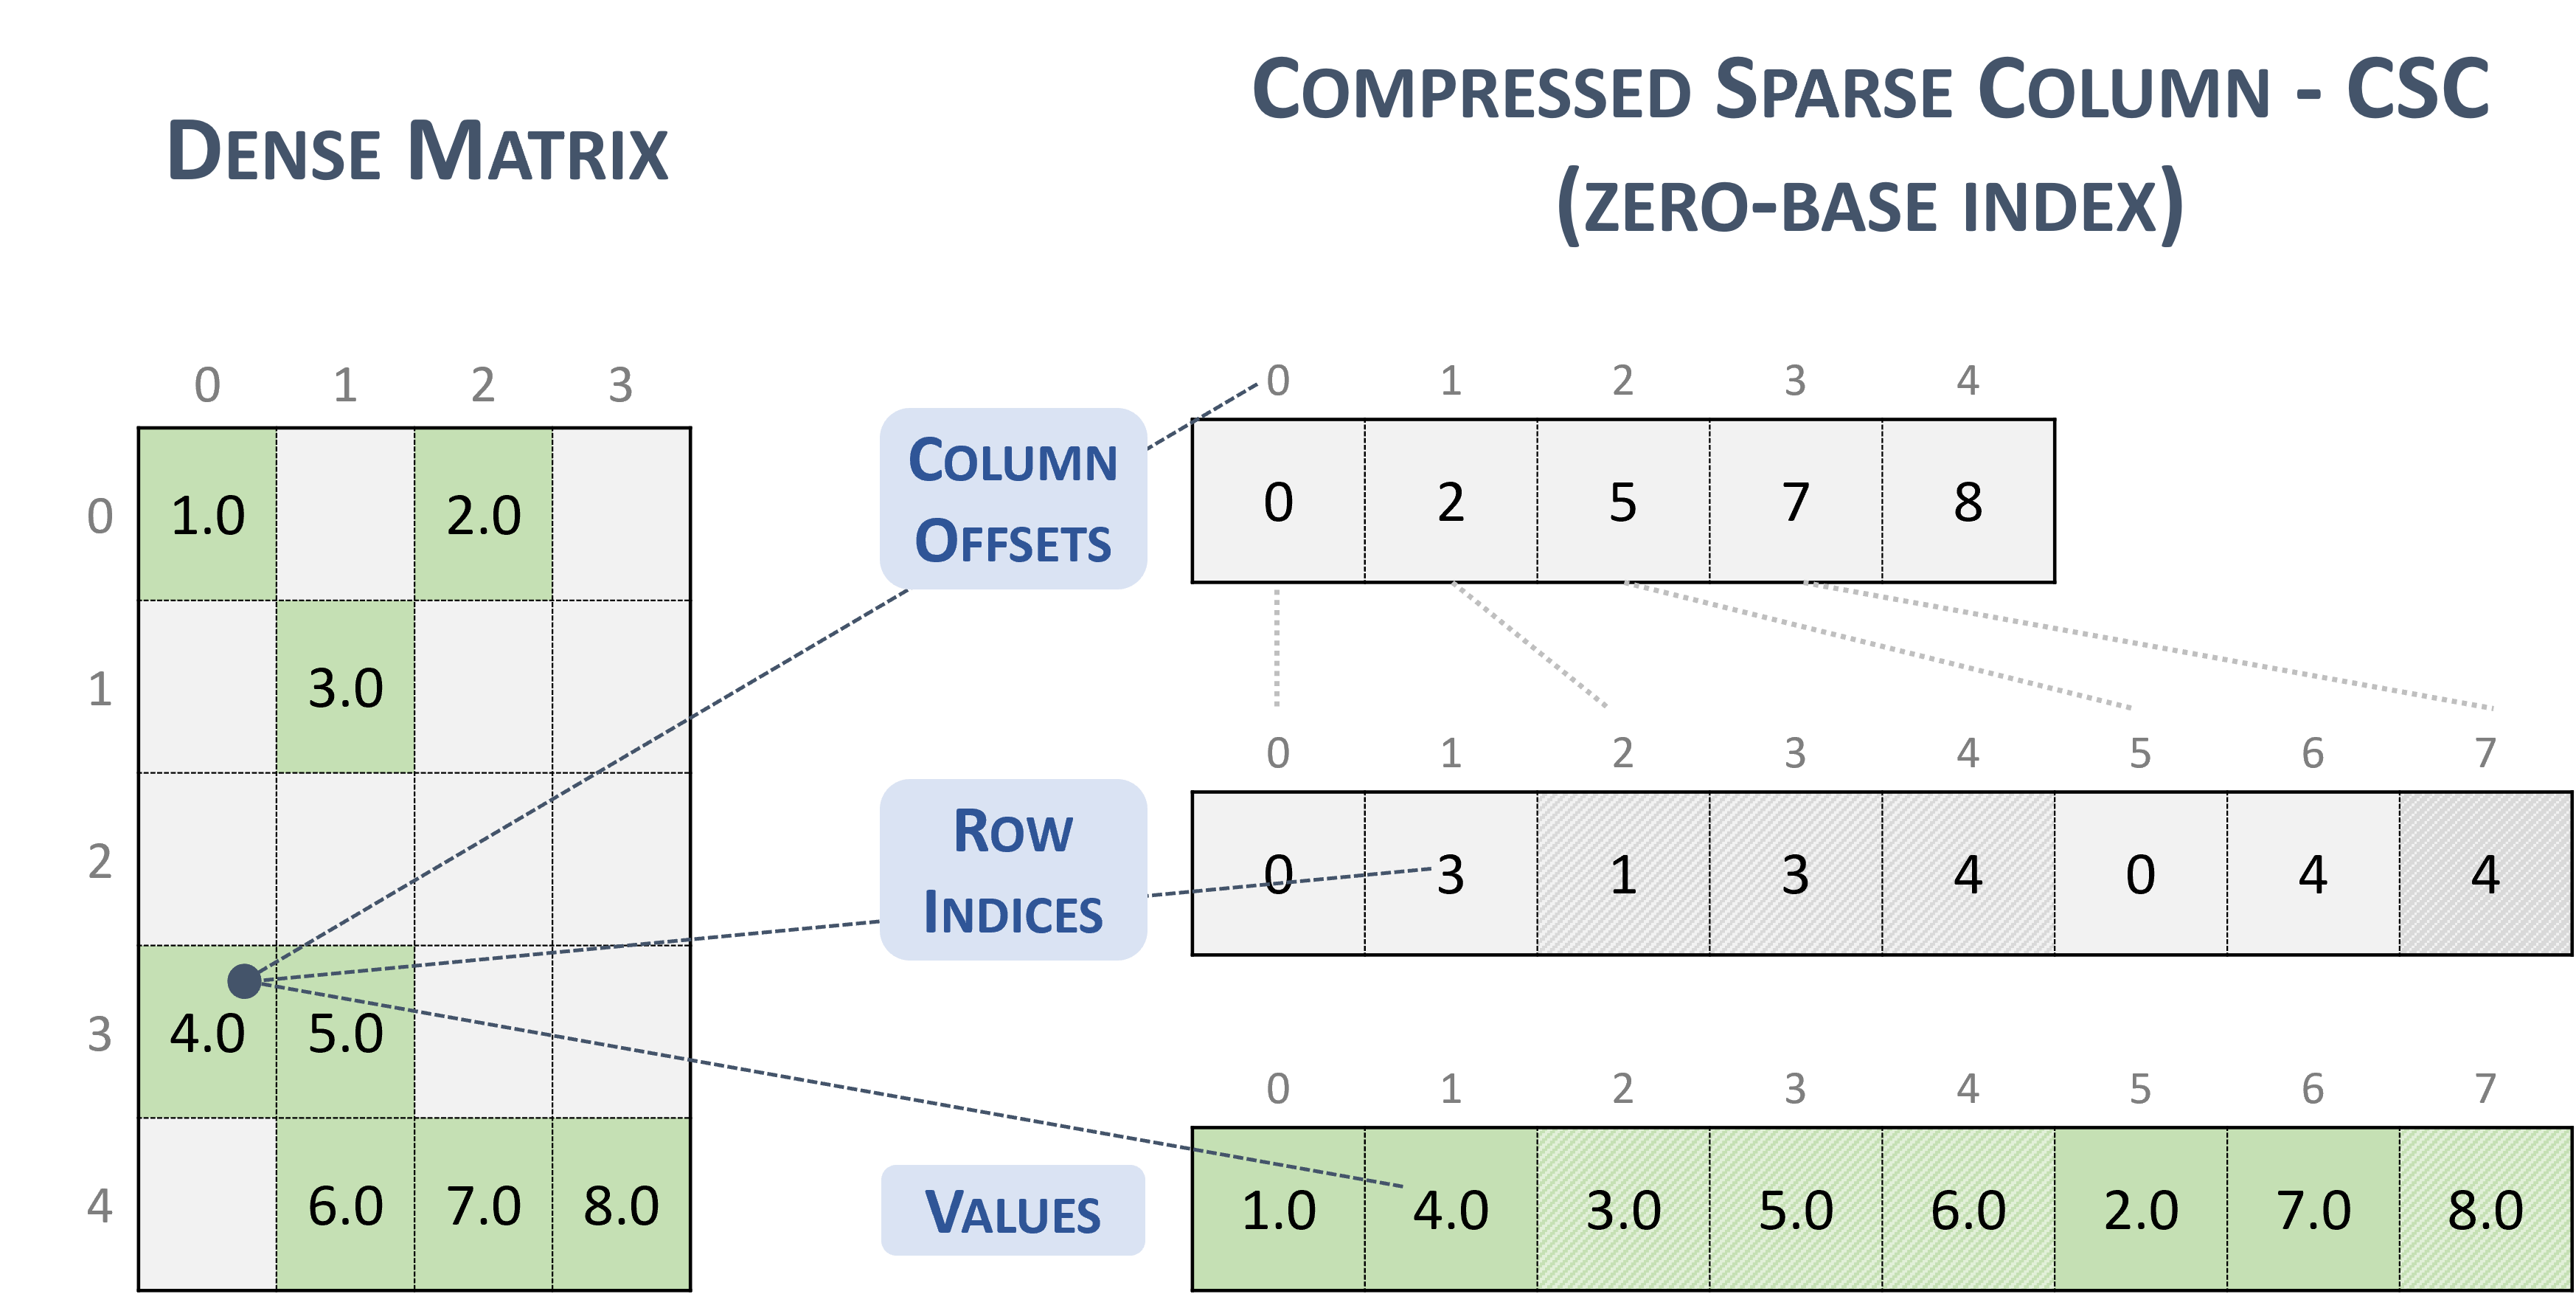
\includegraphics[width=\textwidth]{csc.png}}
\end{frame}
\begin{frame}{Compressed Sparse Column (CSC) Format}
    \begin{itemize}
        \item In the CSC format, the matrix is stored as three arrays: \texttt{values}, \texttt{rows}, and \texttt{col\_ptr}.
       
    \end{itemize}
    \centerline{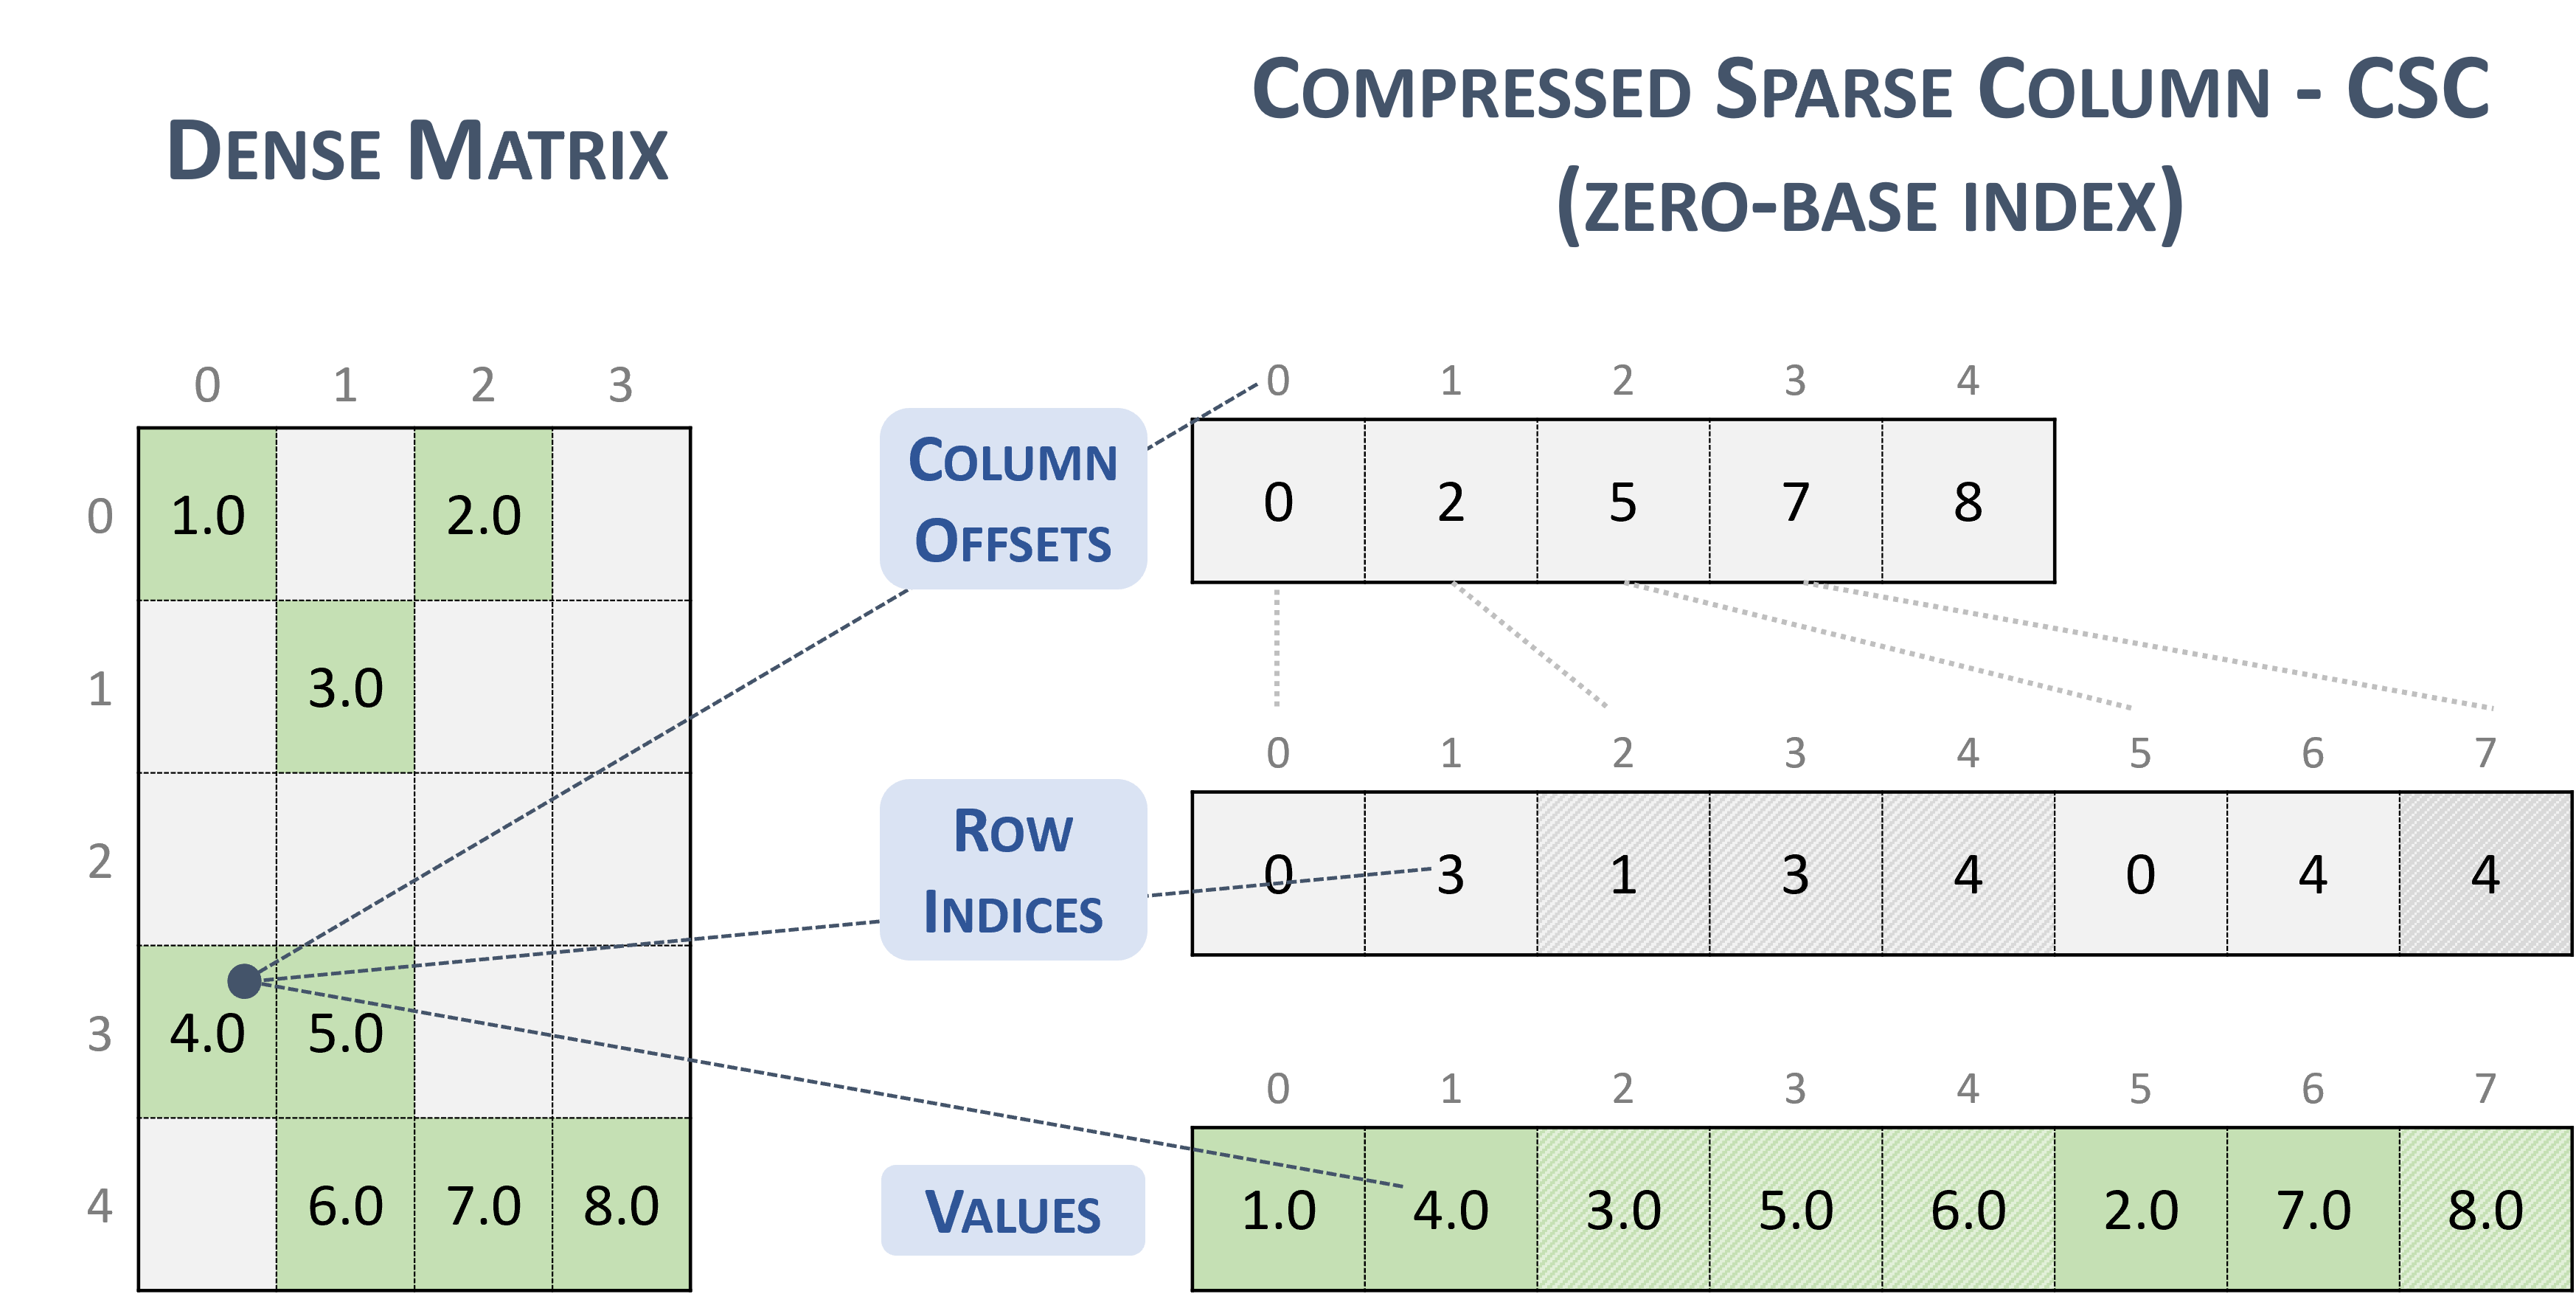
\includegraphics[width=\textwidth]{csc.png}}
\end{frame}
\section{Iterative Methods}
\begin{frame}{Iterative Methods}
    \begin{itemize}
        \item Iterative methods are used to solve linear systems of equations.
        \item The basic idea is to start with an initial guess and iteratively improve the solution.
        \item  Because the required number of iterations can be large, the indirect methods are, in general,
        slower than their direct counterparts. However, they are often more memory efficient and can be used for large-scale problems.
        \item The most common iterative methods are the Jacobi, Gauss-Seidel, and Conjugate Gradient methods.
    \end{itemize}
    
\end{frame}
\begin{frame}{Gauss-Seidel Method}
    \begin{itemize}
    \item We want to solve $\mathbf{Ax}=\mathbf{b}$, or
    $$
    \sum_{i=1}^n A_{i j} x_j=b_i, \quad i=1,2, \ldots, n.
    $$
    \item Extracting the term containing $x_i$
    $$
    A_{i i} x_i+\sum_{\substack{j=1 \\ j \neq i}}^n A_{i j} x_j=b_i, \quad i=1,2, \ldots, n
    $$
    \item Solving for $x_i$, 
    $$
x_i=\frac{1}{A_{i i}}\left(b_i-\sum_{\substack{j=1 \\ j \neq i}}^n A_{i j} x_j\right), \quad i=1,2, \ldots, n
$$
This gives an iteration scheme.
    \end{itemize}
\end{frame}
\begin{frame}{Gauss-Seidel Method}
    \begin{itemize}
        \item If we choose a random vector starting $\mathbf{x}^0$, we can iterate according to  
        $$
x_i^{t+1} \leftarrow \frac{1}{A_{i i}}\left(b_i-\sum_{\substack{j=1 \\ j \neq i}}^n A_{i j} x_j^{t}\right), \quad i=1,2, \ldots, n
$$
until convergence.
    \end{itemize}
\end{frame}
\begin{frame}{Relaxation}
    \begin{itemize}
        \item Convergence of the Gauss-Seidel method can be improved by a technique known
        as \textbf{relaxation}.
        \item We take the  new value of $x_i$ as a weighted average of its previ-
        ous value and the value predicted as above. 
$$
x_i^{t+1} \leftarrow \frac{\omega}{A_{i i}}\left(b_i-\sum_{\substack{j=1 \\ j \neq i}}^n A_{i j} x_j^t\right)+(1-\omega) x_i^t, \quad i=1,2, \ldots, n
$$,
where the weight $\omega$ is called the relaxation factor. 
\item  If $\omega <1$, this is an interpolation between the old $x_i^t$ and the predicted value $x_i^{t+1}$. 
This is called \emph{under-relaxation}.
\item In cases where $\omega > 1$, we have extrapolation, or \emph{over-relaxation}.
    \end{itemize}

\end{frame}

\begin{frame}[fragile]{Algorithm: Gauss-Seidel Method}
\begin{algorithm}[H]
\caption{Gauss-Seidel Method}
\begin{algorithmic}[1]
\State \textbf{Input:} Matrix $\mathbf{A}$, vector $\mathbf{b}$, initial guess $\mathbf{x}^0$, tolerance $\epsilon$, maximum iterations $max\_iter$
\State \textbf{Output:} Solution vector $\mathbf{x}$
\For{$k = 0$ to $max\_iter$}
    \State $\mathbf{x}^{k+1} \gets \mathbf{x}^k$
    \For{$i = 1$ to $n$}
        \State $sum \gets b_i$
        \For{$j = 1$ to $n$}
            \If{$j \neq i$}
                \State $sum \gets sum - A_{ij} \cdot x_j^{k+1}$
            \EndIf
        \EndFor
        \State $x_i^{k+1} \gets \frac{sum}{A_{ii}}$
    \EndFor
    \If{$\|\mathbf{x}^{k+1} - \mathbf{x}^k\| < \epsilon$}
        \State \textbf{break}
    \EndIf
\EndFor
\State \textbf{return} $\mathbf{x}^{k+1}$
\end{algorithmic}
\end{algorithm}
\end{frame}
\begin{frame}{Conjugated Gradient}

    \begin{itemize}
        \item The Conjugate Gradient (CG) method is an algorithm for the numerical solution of particular systems of linear equations, namely those whose matrix is symmetric and positive-definite.
        \item It is an iterative method, meaning it generates a sequence of approximations to the solution.
        \item The method is based on the idea of minimizing the quadratic form associated with the system of linear equations.
        \item The CG method is particularly useful for large sparse systems where direct methods are computationally expensive.
        \item The algorithm proceeds by generating a sequence of search directions that are conjugate with respect to the matrix, ensuring that each step reduces the residual error.
       
    \end{itemize}

\end{frame}
\begin{frame}{Conjugated Gradient}
    \begin{itemize}
        \item Consider the problem of finding vector $\mathbf{x}$ that minimizes the quadratic form
        $$
f(\mathbf{x})=\frac{1}{2} \mathbf{x}^T \mathbf{A x}-\mathbf{b}^T \mathbf{x}
$$
where $\mathbf{A}$ is a symmetric positive-definite matrix.
\item $f(\mathbf{x})$ is minimized when $\nabla f=\mathbf{A x}-\mathbf{b}=0$, or  
\[ 
\mathbf{A x}=\mathbf{b}.
\]
\item The CG methods accomplish the minimization by iteration.
    \end{itemize}

\end{frame}
\begin{frame}{Residual}
\begin{itemize}
    \item  The CG methods accomplish the minimization by iteration, starting with an
    initial vector $\mathbf{x}_0$.
    \item Each iterative cycle $k$ generates a new approximation $\mathbf{x}^k$ to the solution, 
    \[
    \mathbf{x}^{k+1}=\mathbf{x}^k+\alpha_k \mathbf{p}^k
    \]
    where $\mathbf{p}^k$ is the search direction, and $\alpha_k$ is the step size.
    \item The residual is defined as the difference between the right-hand side and the current approximation,
    \[
    \mathbf{r}^k=\mathbf{b}-\mathbf{A x}^k
    \] 
    \item We obtain the solution for $\alpha_k$ by minimizing the quadratic form along the search direction.
    \[
    \alpha_k=\frac{\mathbf{r}^{k,T}  \mathbf{r}^k}{\mathbf{p}^{k,T} \mathbf{A p}^k}
    \]
\end{itemize}
\end{frame}
\begin{frame}{Search Direction}
    \begin{itemize}
        \item The search direction $\mathbf{p}^k$ is chosen to be conjugate to the previous search directions.
        \item The new search direction is given by
        \[
        \mathbf{p}^{k+1}=\mathbf{r}^{k+1}+\beta_k \mathbf{p}^k
        \]
        where $\beta_k$ is chosen to ensure that $\mathbf{p}^{k+1}$ is conjugate to $\mathbf{p}^k$, i.e.,
        \[
        \mathbf{p}^{k+1,T} \mathbf{A p}^k=0.
        \]
        \item Solving for $\beta_k$ gives
        \[
        \beta_k=\frac{\mathbf{r}^{k+1,T} \mathbf{r}^{k+1}}{\mathbf{r}^{k,T} \mathbf{r}^k}
        \]
        \item The CG method generates a sequence of search directions that are conjugate with respect to the matrix $\mathbf{A}$.
        \item This ensures that each step reduces the residual error.
    \end{itemize}

\end{frame}

\begin{frame}[fragile]{Algorithm: Conjugate Gradient Method}
\begin{algorithm}[H]
\caption{Conjugate Gradient Method}
\begin{algorithmic}[1]
\State \textbf{Input:} Matrix $\mathbf{A}$, vector $\mathbf{b}$, initial guess $\mathbf{x}^0$, tolerance $\epsilon$, maximum iterations $max\_iter$
\State \textbf{Output:} Solution vector $\mathbf{x}$
\State $\mathbf{r}^0 \gets \mathbf{b} - \mathbf{A}\mathbf{x}^0$
\State $\mathbf{p}^0 \gets \mathbf{r}^0$
\For{$k = 0$ to $max\_iter$}
    \State $\alpha_k \gets \frac{\mathbf{r}^k \cdot \mathbf{r}^k}{\mathbf{p}^k \cdot \mathbf{A}\mathbf{p}^k}$
    \State $\mathbf{x}^{k+1} \gets \mathbf{x}^k + \alpha_k \mathbf{p}^k$
    \State $\mathbf{r}^{k+1} \gets \mathbf{r}^k - \alpha_k \mathbf{A}\mathbf{p}^k$
    \If{$\|\mathbf{r}^{k+1}\| < \epsilon$}
        \State \textbf{break}
    \EndIf
    \State $\beta_k \gets \frac{\mathbf{r}^{k+1} \cdot \mathbf{r}^{k+1}}{\mathbf{r}^k \cdot \mathbf{r}^k}$
    \State $\mathbf{p}^{k+1} \gets \mathbf{r}^{k+1} + \beta_k \mathbf{p}^k$
\EndFor
\State \textbf{return} $\mathbf{x}^{k+1}$
\end{algorithmic}
\end{algorithm}
\end{frame}
\begin{frame}{Usage of Conjugate Gradient Method}
    \begin{itemize}
        \item The conjugate gradient method is not competitive with direct methods in the solution of small sets of equations.
        \item Its strength lies in the handling of large, sparse systems (where most elements of $\mathbf{A}$ are zero).
        \item Only the matrix-vector product $\mathbf{A}\mathbf{p}^k$ is required, which can be computed efficiently for sparse matrices.
        \item If $\mathbf{A}$ is ill-conditioned, the CG method may converge slowly. It is often used in combination with preconditioning.
    \end{itemize}
    
\end{frame}
\end{document}


